 %%
%%

\section*{Bacula Frequently Asked Questions}
\label{_ChapterStart48}
\index[general]{Questions!Bacula Frequently Asked }
\index[general]{Bacula Frequently Asked Questions }
\addcontentsline{toc}{section}{Bacula Frequently Asked Questions}

See 
\ilink{the bugs section}{_ChapterStart4} of this document for a list
of known bugs and solutions.

\begin{description}
\label{what}

\item [What is {\bf Bacula}? ]
   \index[general]{What is Bacula? }
   {\bf Bacula} is a network backup and restore program. 

\item [Does Bacula support Windows?]
   \index[general]{Does Bacula support Windows? }
   Yes, Bacula compiles and runs on Windows machines  (Win98, WinMe, WinXP,
   WinNT, and Win2000).  We provide a binary version of the Client (bacula-fd),
   but have  not tested the Director nor the Storage daemon. Note, Win95  is no
   longer supported because it doesn't have the  GetFileAttributesExA API call.  

\label{lang}
\item [What language is Bacula written in?]
   \index[general]{What language is Bacula written in? }
   It is written in C++, but it is mostly C  code using only a limited set of the
   C++ extensions  over C.  Thus Bacula is completely  compiled using the C++
   compiler. There are several modules,  including the Win32 interface that are
   written using the  object oriented C++ features. Over time, we are slowly
   adding a larger  subset of C++.  

\label{run}
\item [On what machines does Bacula run? ]
   \index[general]{On what machines does Bacula run? }
   {\bf Bacula} builds and executes on RedHat Linux (versions  RH7.1-RHEL 3.0,
   SuSE, Gentoo, Debian, Mandrake, ...), FreeBSD,  Solaris, Alpha, SGI (client),
   NetBSD, OpenBSD, Mac OS X (client),  and Win32 (client).  

   Bacula has been my only backup tool for over  four years backing up 5 machines
   nightly (3 Linux boxes  running RedHat, a WinXP machine, and a WinNT machine).
 

\label{stable}
\item [Is Bacula Stable? ]
   \index[general]{Is Bacula Stable? }
   Yes, it is remarkably stable, but remember, there are  still a lot of
   unimplemented or partially implemented features.  With a program of this size
   (100,000+ lines of C++ code  not including the SQL programs) there are bound
   to be bugs.  The current test environment (a twisted pair local network and a
   HP DLT  backup tape) is rather ideal, so additional testing on other  sites is
   necessary. The File daemon has never crashed -- running  months at a time with
   no intervention. The Storage daemon is  remarkably stable with most of the
   problems arising during labeling  or switching tapes. Storage daemon crashes
   are rare.  The Director, given the multitude of functions it fulfills is  also
   relatively stable. In a production environment, it rarely  if ever crashes. Of
   the three daemons, the Director is the most  prone to having problems. It
   frequently runs several months with  no problems.  

   There are a number of reasons for this stability.  

   \begin{enumerate}
   \item The program was largely written by one person to date
      (Kern).\\
   \item  The program constantly is checking the chain of allocated
      memory buffers to ensure that no overruns have occurred.  \\
   \item All  memory leaks (orphaned buffers) are reported each time the
      program  terminates.\\
   \item Any signal (segmentation fault, ...) generates a 
      traceback that is emailed to the developer. This permits quick  resolution of
      bugs even if they only show up rarely in a  production system.\\
   \item There is a reasonably comprehensive set of regression tests
      that avoids re-creating the most common errors in new versions of
      Bacula.
   \end{enumerate}

\label{AuthorizationErrors}

\item [I'm Getting Authorization Errors. What is Going On? ]
   \index[general]{I'm Getting Authorization Errors. What is Going On? }
   For security reasons, Bacula requires that both  the File daemon and the
   Storage daemon know the name  of the Director as well as his password. As a
   consequence,  if you change the Director's name or password, you must  make
   the corresponding change in the Storage daemon and  in the File daemon
   configuration files.  

   During the authorization process, the Storage daemon  and File daemon also
   require that the Director authenticate  itself, so both ends require the other
   to have the correct  name and password.  

   If you have edited the conf files and modified any name or  any password, and
   you are getting authentication errors,  then your best bet is to go back to
   the  original conf files generated by the Bacula installation  process. Make
   only the absolutely necessary modifications  to these files -- e.g. add the
   correct email address. Then  follow the instructions in the 
   \ilink{ Running Bacula}{_ChapterStart1} chapter of this manual. You
   will run  a backup to disk and a restore. Only when that works, should you
   begin customization of the conf files.  

   Another reason that you can get authentication errors is  if you are running
   Multiple Concurrent Jobs in the Director,  but you have not set them in the
   File daemon or the Storage  daemon. Once you reach their limit, they will
   reject the  connection producing authentication (or connection) errors.

   If you are having problems connecting to a Windows machine that previously
   worked, you might try restarting the Bacula service since Windows frequently 
   encounters networking connection problems.

   Here is sort of a picture of what names/passwords in which  files/Resources
   must match up:  

   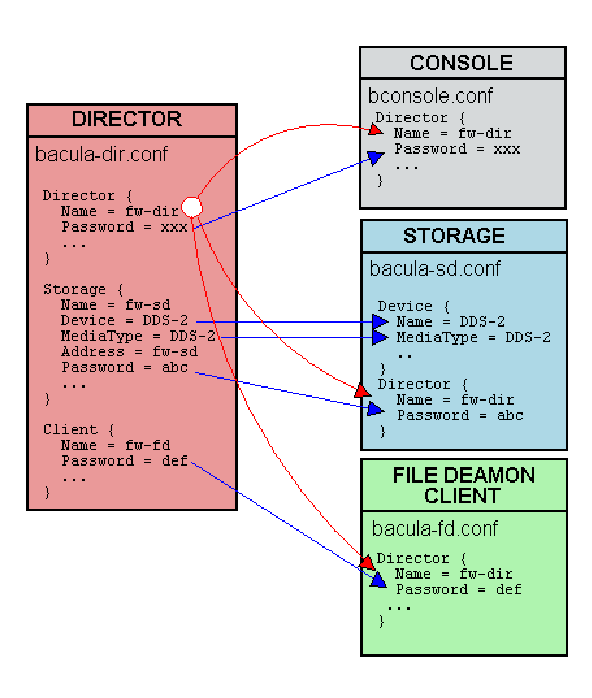
\includegraphics{./Conf-Diagram.eps}  

   In the left column, you will find the Director, Storage, and  Client
   resources, with their names and passwords -- these  are all in {\bf
   bacula-dir.conf}. In the right column  are where the corresponding values
   should be found in the  Console, Storage daemon (SD), and File daemon (FD)
   configuration  files.  

\label{AccessProblems}

\item [Bacula Runs Fine but Cannot Access a Client on a Different Machine.
   Why? ]
   \index[general]{Bacula Runs Fine but Cannot Access a Client on a Different
   Machine. Why? }
   There are several reasons why Bacula could not contact a client  on a
   different machine. They are:  

\begin{itemize}
\item It is a Windows Client, and the client died because of an  improper
   configuration file. Check that the Bacula icon is in  the system tray and the
   the menu items work. If the client has  died, the icon will disappear only
when you move the mouse over  the icon.  
\item The Client address or port is incorrect or not resolved by  DNS. See if
   you can ping the client machine using the same  address as in the Client
   record.  
\item You have a firewall, and it is blocking traffic on port  9102 between
   the Director's machine and the Clients  machine (or on port 9103 between the
   Client and the Storage daemon  machines).  
\item Your password or names are not correct in both the Director and  the
   Client machine. Try configuring everything identical to  how you run the
   client on the same machine as the Director, but  just change the Address. If
that works, make the other changes  one step at a time until it works.  
\end{itemize}

\label{startover}

\item [My Catalog is Full of Test Runs, How Can I Start Over? ]
  \index[general]{My Catalog is Full of Test Runs, How Can I Start Over? }
  If you are using MySQL do the following:

\footnotesize
\begin{verbatim}
   cd <bacula-source>/src/cats
   ./drop_mysql_tables
   ./make_mysql_tables
 
\end{verbatim}
\normalsize

If you are using SQLite, do the following:

\footnotesize
\begin{verbatim}
   Delete bacula.db from your working directory.
   cd <bacula-source>/src/cats
   ./drop_sqlite_tables
   ./make_sqlite_tables
 
\end{verbatim}
\normalsize

Then write an EOF on each tape you used with {\bf Bacula} using: 

\footnotesize
\begin{verbatim}
mt -f /dev/st0 rewind
mt -f /dev/st0 weof
\end{verbatim}
\normalsize

where you need to adjust the device name for your system.  

\label{restorehang}
\item [I Run a Restore Job and Bacula Hangs. What do I do?]
   \index[general]{I Run a Restore Job and Bacula Hangs. What do I do? }
   On Bacula version 1.25 and prior, it expects you to  have the correct tape
   mounted prior to a restore. On  Bacula version 1.26 and higher, it will ask
   you for the  tape, and if the wrong one it mounted, it will inform you.  

   If you have previously done an {\bf unmount} command, all  Storage daemon
   sessions (jobs) will be completely blocked  from using the drive unmounted, so
   be sure to do a {\bf mount}  after your unmount. If in doubt, do a second {\bf
   mount}, it  won't cause any harm.  

\label{windowstart}
\item [I Cannot Get My Windows Client to Start Automatically? ]
   \index[general]{I Cannot Get My Windows Client to Start Automatically? }
   You are probably having one of two problems: either the  Client is dying due
   to an incorrect configuration file, or  you didn't do the Installation
   commands necessary to install  it as a Windows Service.  

   For the first problem, see the next FAQ question. For the  second problem,
   please review the 
   \ilink{ Windows Installation instructions}{_ChapterStart7} in this
   manual.  

\label{windowsdie}

\item [My Windows Client Immediately Dies When I Start It ]
\index[general]{My Windows Client Immediately Dies When I Start It }
The most common problem is either that the configuration  file is not where it
expects it to be, or that there is an  error in the configuration file.  You
must have the configuration file in  {\bf
c:\textbackslash{}bacula\textbackslash{}bin\textbackslash{}bacula-fd.conf}.  

To {\bf see} what is going on when the File daemon starts  on Windows, do the
following:  

\footnotesize
\begin{verbatim}
    Start a DOS shell Window.
    cd c:\bacula\bin
    bacula-fd -d100 -c c:\bacula\bin\bacula-fd.conf
    
\end{verbatim}
\normalsize

This will cause the FD to write a file {\bf bacula.trace}  in the current
directory, which you can examine and determine  the problem.  

\label{scroll}
\item [When I Start the Console, the Error Messages Fly By. How can I see
   them? ]
   \index[general]{When I Start the Console, the Error Messages Fly By. How can I seethem? }
   Either use a shell window with a scroll bar, or use the gnome-console.  In any
   case, you probably should be logging all output to a file, and  then you can
   simply view the file using an editor or the {\bf less}  program. To log all
   output, I have the following in my Director's  Message resource definition:  

\footnotesize
\begin{verbatim}
    append = "/home/kern/bacula/bin/log" = all, !skipped
    
\end{verbatim}
\normalsize

Obviously you will want to change the filename to be appropriate  for your
system.  

\label{nobackup}
\item [I didn't realize that the backups were not working on my Windows 
   Client. What should I do? ]
\index[general]{I didn't realize that the backups were not working on my Windows
Client. What should I do? }
You should be sending yourself an email message for each job. This will  avoid
the possibility of not knowing about a failed backup. To do so  put something
like:  

\footnotesize
\begin{verbatim}
  Mail = yourname@yourdomain = all, !skipped
  
\end{verbatim}
\normalsize

in your Director's message resource. You should then receive one  email for
each Job that ran. When you are comfortable with what  is going on (it took me
9 months), you might change that to:  

\footnotesize
\begin{verbatim}
   MailOnError = yourname@yourdomain = all, !skipped
   
\end{verbatim}
\normalsize

then you only get email messages when a Job errors as is the case  for your
Windows machine.  

You should also be logging the Director's messages, please see the  previous
FAQ for how to do so.  

\label{sched}
\item [All my Jobs are scheduled for the same time. Will this cause
   problems? ]
   \index[general]{All my Jobs are scheduled for the same time. Will this cause
   problems? }
   No, not at all. Bacula will schedule all the Jobs at the same time,  but will
   run them one after another unless you have increased the number  of
   simultaneous jobs in the configuration files for the Director,  the File
   daemon, and the Storage daemon. The appropriate configuration  record is {\bf
   Maximum Concurrent Jobs = nn}. At the current time,  we recommend that you
   leave this set to {\bf 1} for the Director.  

\label{disk}
\item [Can Bacula Backup My System To Files instead of Tape? ]
   \index[general]{Can Bacula Backup My System To Files instead of Tape? }
   Yes, in principle, Bacula can backup to any storage  medium as long as you
   have correctly defined that medium in the  Storage daemon's Device resource.
   For an example of how to backup  to files, please see the  
   \ilink{Pruning Example}{PruningExample} in the  Recycling
   chapter of this manual. Also, there is a whole chapter  devoted to 
   \ilink{Backing Up to Disk}{_ChapterStart39}.  

\label{bigfiles}
\item [Can Bacula Backup and Restore Files Greater than 2 Giga bytes in
   Size?  ]
\index[general]{Can Bacula Backup and Restore Files Greater than 2 Giga bytes in
Size? }
If your operating system permits it, and you are running Bacula  version 1.26
or later, the answer is yes. To the best of our  knowledge all client system
supported by Bacula can handle  files larger than 2 Giga bytes.  

\label{cancel}
\item [I Started A Job then Decided I Really Did Not Want to Run It. Is
   there  a better way than {\bf ./bacula stop} to stop it?]
   \index[general]{I Started A Job then Decided I Really Did Not Want to
   Run It.  Is there a better way than ./bacula stop to stop it?  } Yes,
   you normally should use the Console command {\bf cancel} to cancel a Job
   that is either scheduled or running.  If the Job is scheduled, it will
   be marked for cancellation and will be canceled when it is scheduled to
   start.  If it is running, it will normally terminate after a few
   minutes.  If the Job is waiting on a tape mount, you may need to do a
   {\bf mount} command before it will be canceled.

\label{trademark}
\item [Why have You Trademarked the Name
   Bacula\raisebox{.6ex}{{\footnotesize \textsuperscript{\textregistered}}}?]
\index[general]{Why have You Trademarked the Name
Bacula\textsuperscript{\textregistered}? }
We have trademarked the name Bacula to ensure that all media  written by any
program named Bacula will always be compatible. Anyone  may use the name
Bacula, even in a derivative product as long as it  remains totally compatible
in all respects with the program defined  here.

\label{docversion}
\item [Why is Your Online Document for Version 1.35 of Bacula when the
   Currently  Release Version is 1.34?]
\index[general]{Why is Your Online Document for Version 1.35 of Bacula when the
Currently Release Version is 1.34? }
As Bacula is being developed, the document is also being enhanced, more  often
than not it has clarifications of existing features that  can be very useful
to our users, so we publish the very latest  document. Fortunately it is rare
that there are confusions with  new features.  

If you want to read a document that pertains only to a specific  version,
please use the one distributed in the source code.  

\label{sure}

\item [How Can I Be Sure that Bacula Really Saves and Restores All Files? ]
   \index[general]{How Can I Be Sure that Bacula Really Saves and Restores
   All Files?  } It is really quite simple, but took me awhile to figure
   out how to ``prove'' it.  First make a Bacula Rescue disk, see the
   \ilink{Disaster Recovery Using Bacula}{_ChapterStart38} of this manual.
   Second, you run a full backup of all your files on all partitions.
   Third, you run an Verify InitCatalog Job on the same FileSet, which
   effectively makes a record of all the files on your system.  Fourth, you
   run a Verify Catalog job and assure yourself that nothing has changed
   (well, between an InitCatalog and Catalog one doesn't expect anything).
   Then do the unthinkable, write zeros on your MBR (master boot record)
   wiping out your hard disk.  Now, restore your whole system using your
   Bacula Rescue disk and the Full backup you made, and finally re-run the
   Verify Catalog job.  You will see that with the exception of the
   directory modification and access dates and the files changed during the
   boot, your system is identical to what it was before you wiped your hard
   disk.

\label{upgrade}
\item [I did a Full backup last week, but now in running an Incremental,
   Bacula  says it did not find a FULL backup time, so it did a FULL backup. Why?]
   \index[general]{I did a Full backup last week, but now in running an
   Incremental, Bacula says it did not find a FULL backup time, so it did a
   FULL backup.  Why?  } Before doing an Incremental or a Differential
   backup, Bacula checks to see if there was a prior Full backup of the
   same Job that terminated successfully.  If so, it uses the date that
   full backup started as the time for comparing if files have changed.  If
   Bacula does not find a successfully full backup, it proceeds to do one.
   Perhaps you canceled the full backup, or it terminated in error.  In
   such cases, the full backup will not be successful.  You can check by
   entering {\bf list jobs} and look to see if there is a prior Job with
   the same Name that has Level F and JobStatus T (normal termination).

   Another reason why Bacula may not find a suitable Full backup is that
   every time you change the FileSet, Bacula will require a new Full
   backup.  This is necessary to ensure that all files are properly backed
   up in the case where you have added more files to the FileSet.
   Beginning with version 1.31, the FileSets are also dated when they are
   created, and this date is displayed with the name when you are listing
   or selecting a FileSet.  For more on backup levels see below.

\label{filenamelengths}
\item [How Can You Claim to Handle Unlimited Path and Filename Lengths
   when  All Other Programs Have Fixed Limits?]
   \index[general]{How Can You Claim to Handle Unlimited Path and Filename
   Lengths when All Other Programs Have Fixed Limits?  } Most of those
   other programs have been around for a long time, in fact since the
   beginning of Unix, which means that they were designed for rather small
   fixed length path and filename lengths.  Over the years, these
   restrictions have been relaxed allowing longer names.  Bacula on the
   other hand was designed in 2000, and so from the start, Path and
   Filenames have been keep in buffers that start at 256 bytes in length
   but can grow as needed to handle any length.  Most of the work is
   carried out by lower level routines making the coding rather easy.

\label{unique}
\item [What Is the Really Unique Feature of Bacula?   ]
   \index[general]{What Is the Really Unique Feature of Bacula?  } Well, it
   is hard to come up with unique features when backup programs for Unix
   machines have been around since the 1960s.  That said, I believe that
   Bacula is the first and only program to use a standard SQL interface to
   its catalog database.  Although this adds a bit of complexity and
   possibly overhead, it provides an amazingly rich set of features that
   are easy to program and enhance.  The current code has barely scratched
   the surface in this regard (version 1.31).

   The second feature, which gives a lot of power and flexibility to Bacula
   is the Bootstrap record definition.

   The third unique feature, which is currently (1.30) unimplemented, and
   thus can be called vaporware :-), is Base level saves.  When
   implemented, this will enormously reduce tape usage.

\label{sequence}

\item [If I Do Run Multiple Simultaneous Jobs, How Can I Force One
   Particular  Job to Run After Another Job? ]
\index[general]{If I Do Run Multiple Simultaneous Jobs, How Can I Force One
Particular Job to Run After Another Job? }
Yes, you can set Priorities on your jobs so that they  run in the order you
specify. Please see:  
\ilink{the Priority record}{Priority} in the  Job resource.

\label{nomail}

\item [I Am Not Getting Email Notification, What Can I Do?

   ]
\index[general]{I Am Not Getting Email Notification, What Can I Do? }
The most common problem is that you have not specified a fully  qualified
email address and your bsmtp server is rejecting the mail.  The next most
common problem is that your bsmtp server doesn't like  the syntax on the From
part of the message. For more details on this  and other problems, please see
the 
\ilink{ Getting Email Notification to Work}{email} section of the
Tips chapter  of this manual. The section 
\ilink{ Getting Notified of Job Completion}{notification} of the Tips
chapter may also  be useful. For more information on the {\bf bsmtp} mail
program,  please see 
\ilink{bsmtp in the Volume Utility Tools chapter}{bsmtp} of this
manual.

\label{periods}

\item [I Change Recycling, Retention Periods, or File Sizes in my Pool
   Resource  and they Still Don``t Work.]
  \index[general]{I Change Recycling, Retention Periods, or File Sizes in my Pool
  Resource and they Still Don"t Work. }
  The different variables associated with a Pool are defined in the  Pool
  Resource, but are actually read by Bacula from the Catalog database.  On
  Bacula versions prior to 1.30, after changing your Pool Resource,  you must
  manually update the corresponding values in the Catalog by  using the {\bf
  update pool} command in the Console program. In Bacula  version 1.30, Bacula
  does this for you automatically every time it  starts.  
  
  When Bacula creates a Media record (Volume), it uses many default  values from
  the Pool record. If you subsequently change the Pool  record, the new values
  will be used as a default for the next Volume  that is created, but if you
  want the new values to apply to existing  Volumes, you must manually update
  the Volume Catalog entry using  the {\bf update volume} command in the Console
  program. 

\label{CompressionNotWorking}
\item [I Have Configured Compression On, But None of My Files Are
   Compressed.  Why?]
   \index[general]{I Have Configured Compression On, But None of My Files Are
   Compressed. Why? }
   There are two kinds of compression. One is tape compression. This  is done by
   the tape drive hardware, and you either enable or disable  it with system
   tools such as {\bf mt}. This compression works  independently of Bacula.  
   
   Bacula also has compression code, which is normally used only when  backing up
   to file Volumes. There are two conditions for this  ''software`` to be
   enabled.  

\begin{enumerate}
\item You must have the zip development libraries loaded on your  system when
   building Bacula and Bacula must find this library,  normally {\bf
   /usr/lib/libz.a}. On RedHat systems, this library  is provided by the {\bf
   zlib-devel} rpm.  

 If the library is found by Bacula during the {\bf ./configure}  it will be
 in dicated on the {\bf config.out} line by:  

\footnotesize
\begin{verbatim}
             ZLIB support:  yes
          
\end{verbatim}
\normalsize

\item You must add the {\bf compression=gzip} option on your  Include
   statement in the Director's configuration file.  
\end{enumerate}

\label{NewTape}
\item [Bacula is Asking for a New Tape After 2 GB of Data but My Tape
   holds 33 GB. Why?]
\index[general]{Bacula is Asking for a New Tape After 2 GB of Data but My Tape
holds 33 GB. Why? }
There are several reasons why Bacula will request a new tape.  

\begin{itemize}
\item There is an I/O error on the tape. Bacula prints an error message  and
   requests a new tape. Bacula does not attempt to continue writing  after an I/O
   error.  
\item Bacula encounters and end of medium on the tape. This is not always 
   distinguishable from an I/O error.  
\item You have specifically set some size limitation on the tape. For  example
   the {\bf Maximum Volume Bytes} or {\bf Maximum Volume Files}  in the
   Director's Pool resource, or {\bf Maximum Volume Size} in  the Storage
  daemon's Device resource.  
\end{itemize}

\label{LevelChanging}

\item [Bacula is Not Doing the Right Thing When I Request an Incremental
   Backup. Why?]
   \index[general]{Bacula is Not Doing the Right Thing When I Request an Incremental
   Backup. Why? }
   As explained in one of the previous questions, Bacula will automatically 
   upgrade an Incremental or Differential job to a Full backup if it cannot  find
   a prior Full backup or a suitable Full backup. For the gory details  on
   how/when Bacula decides to upgrade levels please see the  
   \ilink{Level record}{Level} in the Director's  configuration
   chapter of this manual.  
   
   If after reading the above mentioned section, you believe that Bacula  is not
   correctly handling the level (Differential/Incremental),  please send us the
   following information for analysis:  

\begin{itemize}
\item Your Director's configuration file.  
\item The output from {\bf list jobs} covering the period where you  are
   having the problem.  
\item The Job report output from the prior Full save (not critical).  
\item An {\bf llist jobid=nnn} where nnn is the JobId of the prior  Full save.
 
\item The Job report output from the save that is doing the  wrong thing (not
   critical).  
\item An {\bf llist jobid=nnn} where nnn is the JobId of the job  that was not
   correct.  
\item An explanation of what job went wrong and why you think it did.  
   \end{itemize}

The above information can allow us to analyze what happened, without it, 
there is not much we can do.  

\label{WaitForever}
\item [I am Backing Up an Offsite Machine with an Unreliable Connection.
   The  Director Waits Forever for the Client to Contact the SD. What Can  I Do.]
   \index[general]{I am Backing Up an Offsite Machine with an Unreliable Connection.
   The Director Waits Forever for the Client to Contact the SD. What Can I Do. }
   Bacula was written  on the assumption that it will have a good TCP/IP
   connection  between all the daemons. As a consequence, the current  Bacula
   doesn't deal with faulty connection very well. This situation  is slowly being
   corrected over time.  
   
   There are several things you can do to improve the situation.  

\begin{itemize}
\item Upgrade to version 1.32 and use the new SDConnectTimeout record.  For
   example, set:  

\footnotesize
\begin{verbatim}
          SD Connect Timeout = 5 min
          
\end{verbatim}
\normalsize

in the FileDaemon resource.  
\item Run these kinds of jobs after all other jobs.  
   \end{itemize}

\label{sshHanging}
\item [When I ssh into a machine and start Bacula then attempt to exit, 
   ssh hangs forever.]
   \index[general]{When I ssh into a machine and start Bacula then attempt to exit,
   ssh hangs forever. }
   This happens because Bacula leaves stdin, stdout, and stderr open  for debug
   purposes. To avoid it, the simplest thing to do is to  redirect the output of
   those files to {\bf /dev/null} or another  file in your startup script (the
   RedHat autostart scripts do this  automatically). For example, you start the
   Director with:  
   
\footnotesize
\begin{verbatim}
    bacula-dir -c bacula-dir.conf ... 0>\&1 2>\&1 >/dev/null
    
\end{verbatim}
\normalsize

and likewise for the other daemons.  

\label{RetentionPeriods}

\item [I'm confused by the different Retention periods: File Retention, 
   Job Retention, Volume Retention. Why are there so many?]
   \index[general]{I'm confused by the different Retention periods: File Retention,
   Job Retention, Volume Retention. Why are there so many? }
   Yes, this certainly can be confusing. The basic reason for so many  is to
   allow flexibility. The File records take quite a lot of space  in the catalog,
   so they are typically records you want to remove  rather quickly. The Job
   records, take very little space, and they  can be useful even without the File
   records to see what Jobs actually  ran and when. One must understand that if
   the File records are removed  from the catalog, you cannot use the {\bf
   restore} command to restore  an individual file since Bacula no longer knows
   where it is. However,  as long as the Volume Retention period has not expired,
   the data will  still be on the tape, and can be recovered from the tape.  
   
   For example, I keep a 30 day retention period for my Files to  keep my catalog
   from getting too big, but I keep my tapes for a  minimum of one year, just in
   case.  

\label{MaxVolumeSize}
\item [Why Does Bacula Ignore the MaxVolumeSize Set in my Pool?]
   \index[general]{Why Does Bacula Ignore the MaxVolumeSize Set in my Pool? }
   The MaxVolumeSize that Bacula uses comes from the Media record,  so most
   likely you changed your Pool, which is used as the default  for creating Media
   records, {\bf after} you created your Volume. Check  what is in the Media
   record by doing: 

\footnotesize
\begin{verbatim}
llist Volume=xxx
\end{verbatim}
\normalsize

If it doesn't have the right value, you can use: 

\footnotesize
\begin{verbatim}
update Volume=xxx
\end{verbatim}
\normalsize

to change it.  

\label{ConnectionRefused}
\item [In connecting to my Client, I get ''ERR:Connection Refused.  Packet
   Size too big from File daemon:192.168.1.4:9102`` Why?]
   \index[general]{In connecting to my Client, I get &htmlQuoteERR:Connection Refused.
   Packet Size too big from File daemon:192.168.1.4:9102&htmlQuote Why? }
   This is typically a communications error resulting  from one of the following:
 

\begin{itemize}
\item Old versions of Bacula, usually a Win32 client, where two  threads were
   using the same I/O packet. Fixed in more recent  versions. Please upgrade.  
\item Some other program such as an HP Printer using the same  port (9102 in
   this case).  
\end{itemize}

If it is neither of the above, please submit a bug report at  
\elink{bugs.bacula.org}{http://bugs.bacula.org}.  

Another solution might be to run the daemon with the debug  option by:  

\footnotesize
\begin{verbatim}
    Start a DOS shell Window.
    cd c:\bacula\bin
    bacula-fd -d100 -c c:\bacula\bin\bacula-fd.conf
    
\end{verbatim}
\normalsize

This will cause the FD to write a file {\bf bacula.trace}  in the current
directory, which you can examine and determine  the problem.  

\end{description}
